\subsection{Sub-project for Keck Foundation support}

\begin{figure}[H]
  \centering
  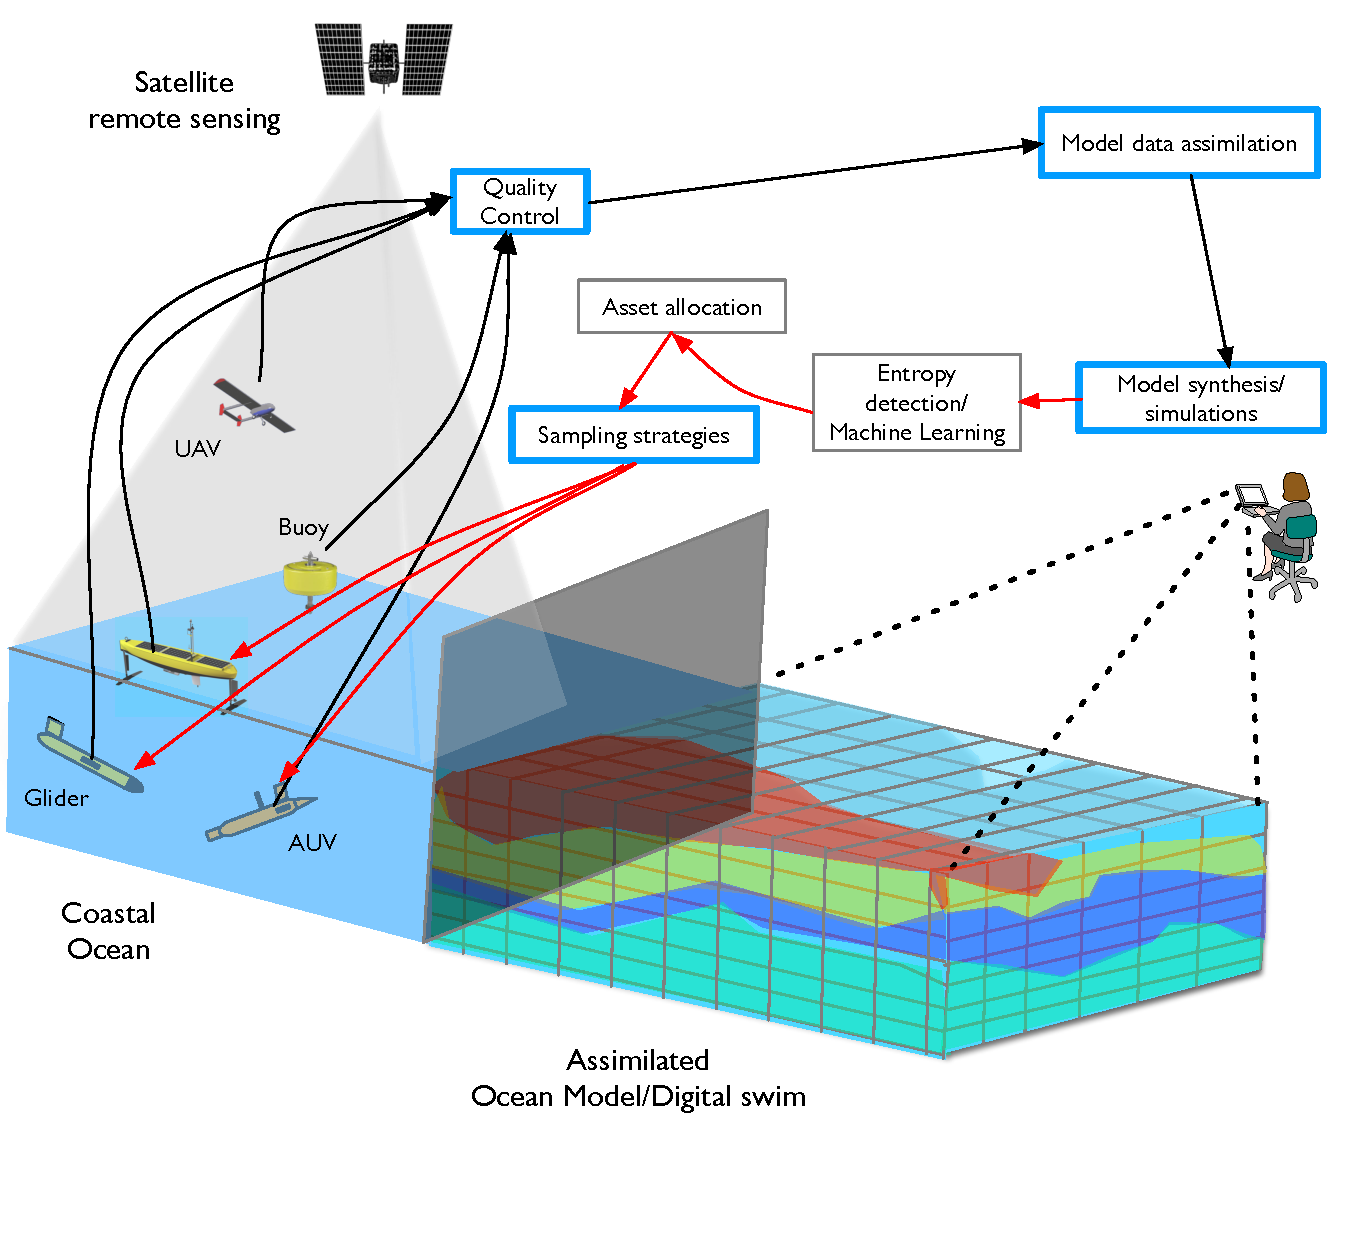
\includegraphics[scale=0.6]{fig/Audacious-pilot-block-diag-2.pdf}
  \caption{A representation of the technical tasks related to \proe. For
    the \kck the tasks related to model assimilation include portions of
    the boxes at the top of the figure in {\color{blue}{blue}}
    outline. Control aspects relate to using the assimilated ocean model
    to focus where and how autonomous platforms will make observation in
    the coastal ocean.}
    \label{fig:block-diag}
\end{figure}

For the \kcke, \pro proposes to focus tasks to those related to model
assimilation and control of autonomous robotic platforms. All
individuals associated with these efforts will be US-based.
Fig. \ref{fig:block-diag} shows the associated tasks highlighted in
{\color{blue}{blue}} and include:

\begin{description}

\item[Automated Data Pipeline, Quality Control \& Assimilation] For
  rapid multi-platform data assimilation and to ensure that the data is
  consistent with expectations of values. This will involve building a
  data pipeline and support infrastructure to ensure that any
  oceanographic sensor or robotic platform can feed data into our ocean
  model ready for assimilation. This task will require a software
  engineer with requisite skills related to data understanding,
  databases, ocean data formats.

\item[Ocean Data Modeler] To make model predictions, \pro will select
  from a range of modeling approaches, focus the domain of the model to
  an area where a proposed field experiment can demonstrate the concepts
  in the 'real world'. The modeler's task will be to initialize the
  model with the geographical conditions of the selected domain
  including the benthic topology and prime the model with remote sensing
  data adequate to initialize conditions for subsequent predictions.

\item[Prediction and Sampling Convergence] Using Bayesian predictive
  capabilities, \pro will pull together a methodology to narrow the
  prediction and sensing gap, between what is sensed in the real-world
  and what was predicted by our model. Strategies to close the expected
  gap will require the use of Machine Learning and Statistical
  techniques, to ensure that robotic platforms can observe in ways to
  bring about convergence. 

\item[Bio-geochemical modeler] Most models incorporate ocean dynamics
  and the physics related to water flow in the context of external
  forcings such as topology, wind, currents and fresh water inflow into
  the ocean. To make a realistic biological impact assessment of these
  dynamics, the variables associated with nutrients transport from the
  benthic as well as riverine environments, those derived from mixing
  and stirring in the upper water-column as well as natural and
  anthropogenic change need to be incorporated into the ocean
  model. This requires a specialist who can understand not only the
  biology, but also the physics of nutrient transport and evolution over
  space and time.

\item[Robotic Sampling Algorithm developer] To ``intelligently'' sample
  the upper water-column, marine robotic vehicles require the
  implementation of algorithms which can sample a wide range of coastal
  ocean phenomenon of interest including Harmful Algal Blooms, plumes,
  oil slicks and hypoxic zones. Using sensor data to craft algorithms
  embedded on AUVs, ASVs and potentially UAVs will require expertise in
  Statistical Sampling and autonomous decision-making and Control. \pro
  will ensure that the latest Sampling methods are embedded for
  computation on robotic vehicles.

\end{description}

\noindent
In addition to supporting the above tasks, \kck funding will help
support the guidance of these personnel by US based PI's. Some support
for instrumentation for use on robotic platform will also be requested
as part of this request.  A near-term goal would be to demonstrate the
development effort in a field experiment to show how a small subset of
the activities and tasks related to \pro can make an impact to the way
scientists sample the coastal ocean. To support this experimentation, a
small ($\sim 10\%$) of the support will be sent to the Univ. of Porto,
Portugal. Doing so would allow the team to position \pro to obtain
further support to fulfill the ambition of the entire proposed project
in this document.

